\documentclass[11pt]{article} 
\usepackage[utf8]{inputenc}

%%% PAGE DIMENSIONS
\usepackage{geometry}
\geometry{a4paper}

\usepackage{graphicx} % support the \includegraphics command and options

% \usepackage[parfill]{parskip} % Activate to begin paragraphs with an empty line rather than an indent

%%% PACKAGES
\usepackage{float}
\usepackage{booktabs}
\usepackage{array}
\usepackage{paralist}
\usepackage{verbatim}
\usepackage{subfig} 
\usepackage{fancyhdr}
\usepackage{amsmath}
\usepackage{amssymb}
\usepackage{hyperref}

\pagestyle{fancy} % options: empty , plain , fancy
\renewcommand{\headrulewidth}{0pt} % customise the layout...
\lhead{}\chead{}\rhead{}
\lfoot{}\cfoot{\thepage}\rfoot{}

\usepackage{sectsty}
\allsectionsfont{\sffamily\mdseries\upshape}

\usepackage{listings}
\usepackage{color}

\definecolor{mygreen}{rgb}{0,0.6,0}
\definecolor{mygray}{rgb}{0.5,0.5,0.5}
\definecolor{mymauve}{rgb}{0.58,0,0.82}
\hypersetup{
    colorlinks=true,
    linkcolor=blue,
    filecolor=magenta,      
    urlcolor=cyan
}
\lstset{ 
  backgroundcolor=\color{white},   % choose the background color; you must add \usepackage{color} or \usepackage{xcolor}; should come as last argument
  basicstyle=\footnotesize,        % the size of the fonts that are used for the code
  breakatwhitespace=false,         % sets if automatic breaks should only happen at whitespace
  breaklines=true,                 % sets automatic line breaking
  captionpos=b,                    % sets the caption-position to bottom
  commentstyle=\color{mygreen},    % comment style
  firstnumber=1000,                % start line enumeration with line 1000
  frame=single,	                   % adds a frame around the code
  keepspaces=true,                 % keeps spaces in text, useful for keeping indentation of code (possibly needs columns=flexible)
  keywordstyle=\color{blue},       % keyword style
  language=Python,                 % the language of the code
  numbers=left,                    % where to put the line-numbers; possible values are (none, left, right)
  numbersep=5pt,                   % how far the line-numbers are from the code
  numberstyle=\tiny\color{mygray}, % the style that is used for the line-numbers
  rulecolor=\color{black},         % if not set, the frame-color may be changed on line-breaks within not-black text (e.g. comments (green here))
  showspaces=false,                % show spaces everywhere adding particular underscores; it overrides 'showstringspaces'
  showstringspaces=false,          % underline spaces within strings only
  showtabs=true,                   % show tabs within strings adding particular underscores
  stepnumber=1,                    % the step between two line-numbers. If it's 1, each line will be numbered
  stringstyle=\color{mymauve},     % string literal style
  tabsize=2,	                   % sets default tabsize to 2 spaces
  title=\lstname                   % show the filename of files included with \lstinputlisting; also try caption instead of title
}


\title{Aprendizaje Automático y Minería de Datos: Proyecto Final}
\author{Ana Martín Sánchez, Nicolás Pastore Burgos\\ \href{https://github.com/NicoPast/AA}{Repositorio en GitHub}}
\date{21/09/2021} 

\begin{document}
\maketitle

\section{Propuesta de proyecto}

	Nuestro proyecto consiste en clasificar setas como comestibles o venenosas, dependiendo de un total de 20 atributos, como los siguientes:
\begin{itemize}
\item  Diámetro del sombrero: un float que representa el diámetro, en cm.
\item  Forma del sombrero: un char que representa una de las posibles formas.
\item  Superficie del sombrero: un char que representa el adjetivo que mejor describe la superficie del sombrero.
\end{itemize}
	
    Para poder analizar los datos, desplegamos algunos de estos atributos (los que eran de tipo enumerado) a matrices de booleanos. Después de esta operación, cada entrada de la base de datos tenía 122 atributos.

	La base de datos tiene un total de 61069 entradas. Por este motivo, no hemos utilizado todos los datos para el proyecto; para las pruebas, de manera general, hemos escogido un 20\% de los datos para entrenar los sistemas, otro 20\% para validarlos y otro 20\% para hacer la prueba final.
    
    La base de datos original, extraída de la plataforma \href{https://www.kaggle.com/dhinaharp/mushroom-dataset }{Kaggle}, tenía los datos organizados de manera que escoger una muestra en el orden establecido no era útil. Por esta razón, decidimos utilizar los datos según estaban organizados en \href{https://mushroom.mathematik.uni-marburg.de/files/}{este repositorio}, ya que estaban mezclados. 
    
    Para entender mejor los datos, presentamos una serie de gráficos que permiten hacer comparaciones entre las setas comestibles y las venenosas:
   
 \begin{figure}[H]
    \begin{center}
    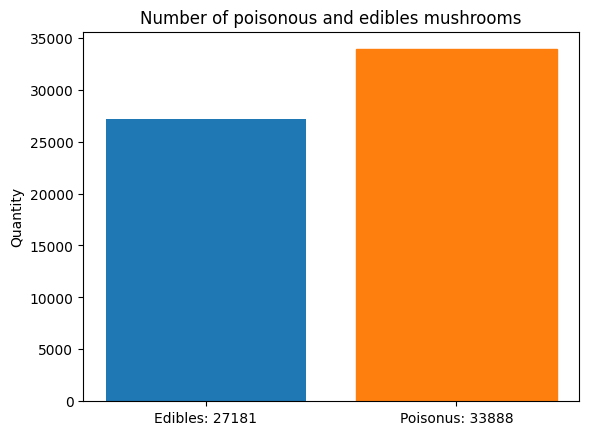
\includegraphics[width=0.6\textwidth]{Results/Analysis/00EdiblesNumb.png}
    \end{center}
 \end{figure}
    Como se puede observar, la cantidad de muestras de setas venenosas supera en número a la de setas comestibles, en más de 6000 entradas.
 
 \begin{figure}[H]
    \begin{center}
    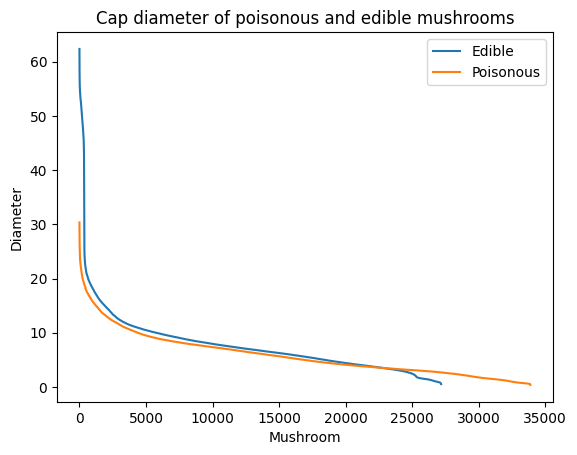
\includegraphics[width=0.6\textwidth]{Results/Analysis/01CapDiameter.png}
    \end{center}
 \end{figure}
	Nos pareció interesante mostrar cómo, cuando el diámetro del sombrero de las setas es muy grande, es muy probable que las setas sean comestibles. Sin embargo, en tamaños intermedios, resulta más difícil diferenciar las setas comestibles de las venenosas.

 \begin{figure}[H]
    \begin{center}
    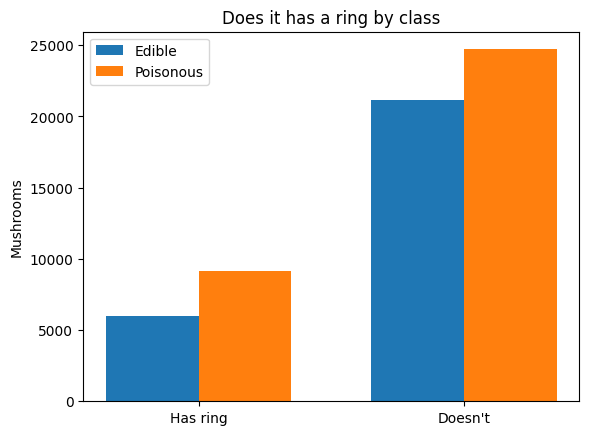
\includegraphics[width=0.6\textwidth]{Results/Analysis/16HasRing.png}
    \end{center}
 \end{figure}
 
	En este caso, vemos que la mayoría de las setas no tienen anillo. Hemos escogido esta gráfica como muestra de algunos de los valores binarios que se van a analizar más adelante.
    
 \begin{figure}[H]
    \begin{center}
    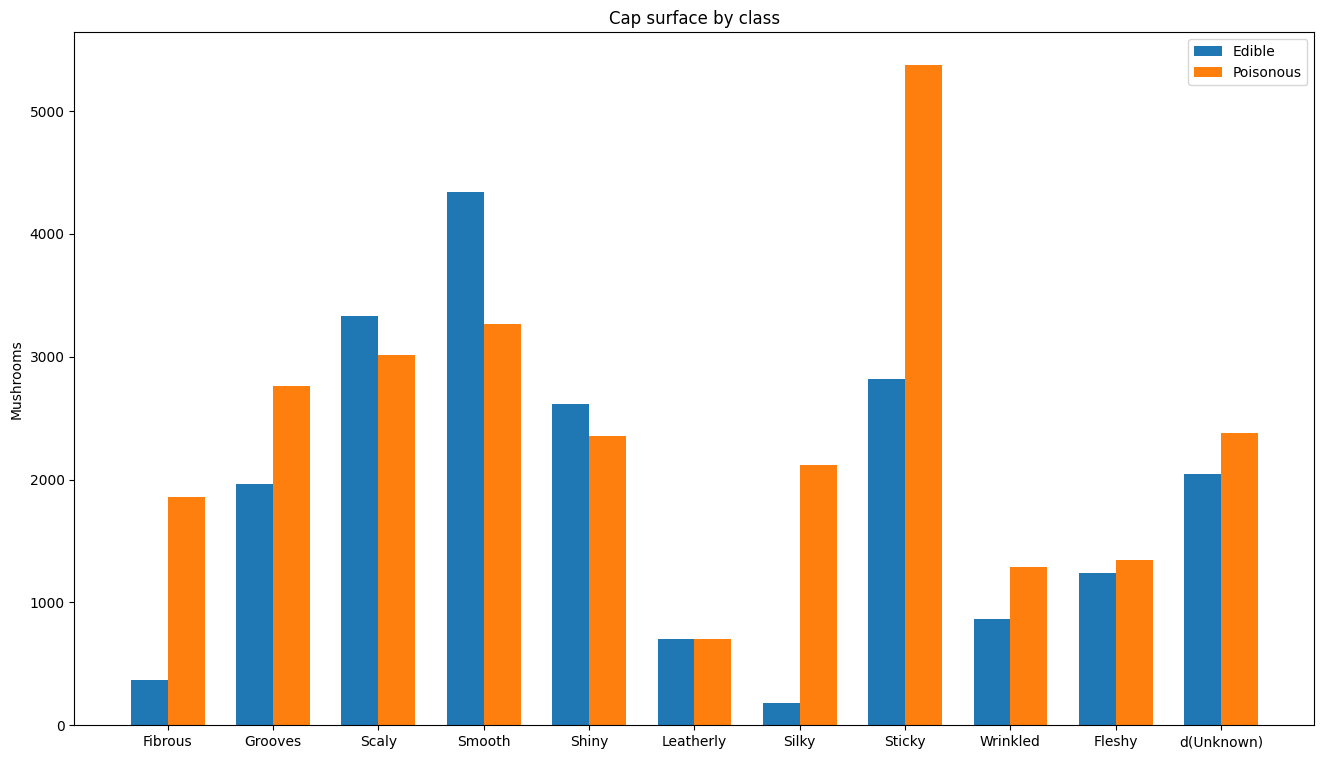
\includegraphics[width=\textwidth]{Results/Analysis/03CapSurface.png}
    \end{center}
 \end{figure}

Por último, se muestran una serie de adjetivos que describen más fiablemente el tipo de superficie del sombrero, y cuáles son venenosas y comestibles. Como se puede ver, y como comentamos a continuación, muchas de las entradas tenían un valor "d" para esta característica (un valor desconocido).

\newpage
\subsection{Problemas encontrados}

Al analizar los datos, nos dimos cuenta de que la base de datos nos supondría algunos problemas para realizar el proyecto:

En primer lugar, hay columnas en las que todos los valores son 0. También se dio que, en la gran mayoría de filas, alguna de las columnas no tenía un valor. 

Por otra parte, algunos de los datos eran contradictorios. En concreto, algunas de las entradas tenían marcado como "t" la columna de has-ring (lo que significa que, efectivamente, tienen un anillo); pero, posteriormente, en la columna de ring-type, tenían marcado "f" (que se corresponde con el tipo "ninguno"). Esto no supone un problema a la hora de implementar los sistemas de aprendizaje automático, pero sí son un problema desde el punto de vista semántico, y nos hacen dudar de la validez de los datos.

 \begin{figure}[H]
    \begin{center}
    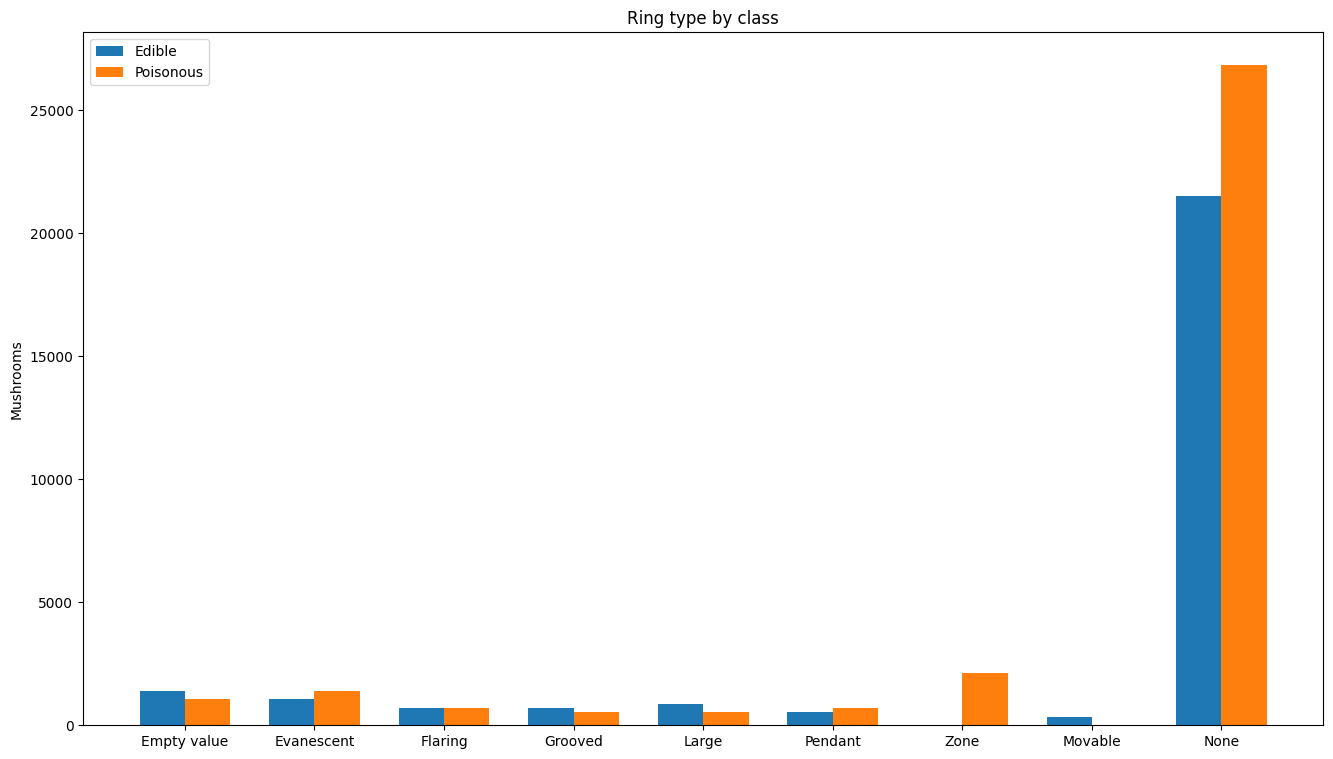
\includegraphics[width=\textwidth]{Results/Analysis/17RingType.png}
    \end{center}
 \end{figure}

Por último, encontramos un problema con la correlación entre los datos y la salida. Como se puede observar en las siguientes gráficas, ninguna de las entradas tiene una correlación que supere el 0.2, ni en el eje positivo ni en el negativo. 

 \begin{figure}[H]
    \begin{center}
    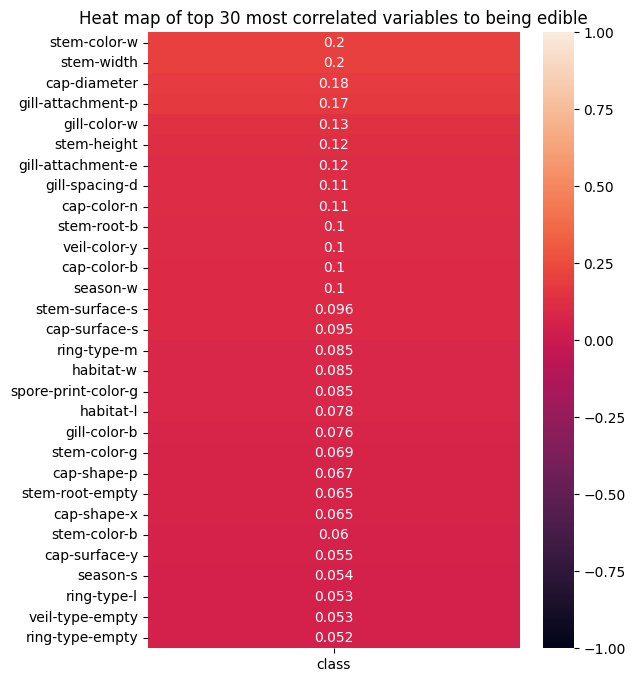
\includegraphics[width=0.7\textwidth]{Results/Analysis/heatMap30Best.png}
    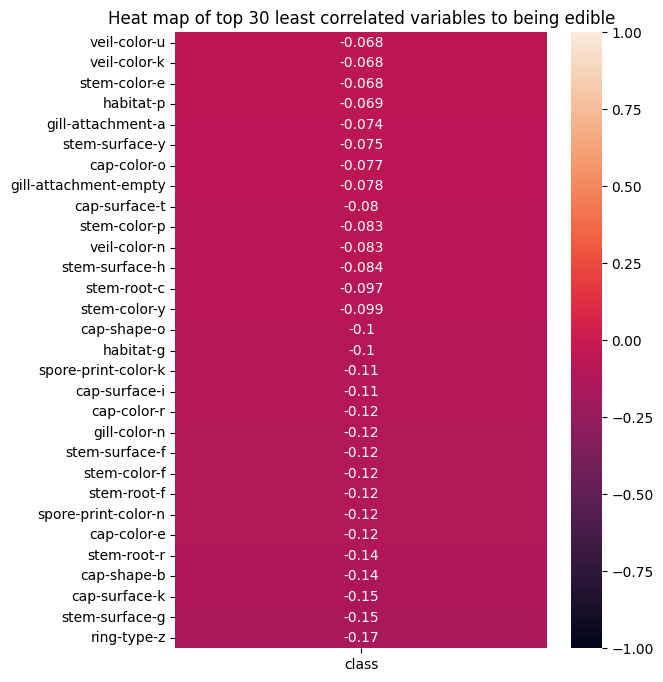
\includegraphics[width=0.7\textwidth]{Results/Analysis/heatMap30Worst.png}
    \end{center}
 \end{figure}
 
 
\newpage
\section{Resultados obtenidos}

Para obtener los mejores resultados posibles, hemos utilizado varios métodos de los estudiados en clase, a fin de poder compararlos. 

\subsection {Regresión Logística}

La regresión logística se puede entender como un caso especial de la regresión lineal, en la que la variable dependiente puede tomar dos valores: 0 o 1. Se emplea para calcular probabilidades (ya que los valores obtenidos estarán entre 0 y 1), o para clasificar eventos en dos categorías; en este caso, se puede utilizar para calcular la probabilidad de que una seta sea comestible (o, dicho de otra manera, para clasificar una seta como comestible o venenosa).

Para utilizar este método, implementamos la función de gradiente, de coste y la función sigmoide como hemos visto en clase, y obtuvimos una tasa de aciertos del 97.14262\%, con un coste de 0.12467. Para llegar a estos resultados, utilizamos un valor para lambda = 3.0 y un exponente = 2.

 \begin{figure}[H]
    \begin{center}
    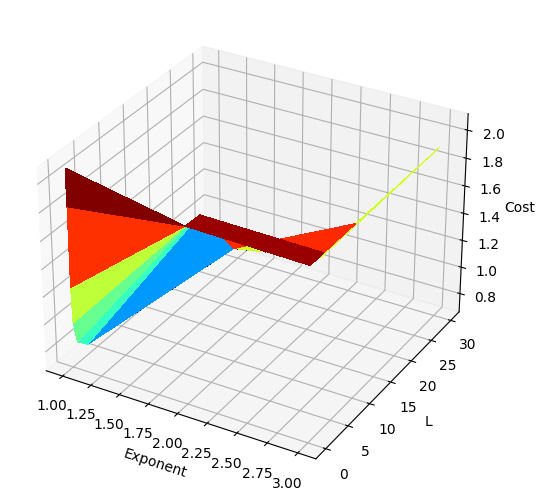
\includegraphics[width=0.45\textwidth]{Results/LogReg/LOG_1.png}
    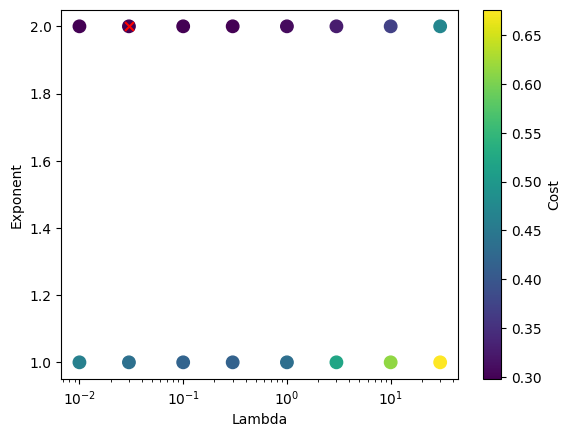
\includegraphics[width=0.45\textwidth]{Results/LogReg/LOG_2.png}
    \end{center}
 \end{figure}

\subsection{Redes Neuronales}

Se entiende como red neuronal a un conjunto de capas ocultas, una capa de entrada y una capa de salida que intentan imitar el funcionamiento del cerebro humano. Cada nodo de las capas (el que equivaldría a una "neurona artificial"), se conecta a otros, y tiene un peso y umbral asociados. Si el valor de un nodo supera su umbral, la "neurona" se activa y envía los datos a la siguiente capa de la red. 

Tras probar con varias configuraciones para la red neuronal, llegamos a un porcentaje de aciertos del 99.828\%, con un coste de 0.0025. Para ello, utilizamos una red neuronal con dos capas ocultas (la primera, con 60 nodos; y la segunda, con 40), y una constante de regularización de 0.3. El algoritmo dio 1000 vueltas para llegar a este resultado.

 \begin{figure}[H]
    \begin{center}
    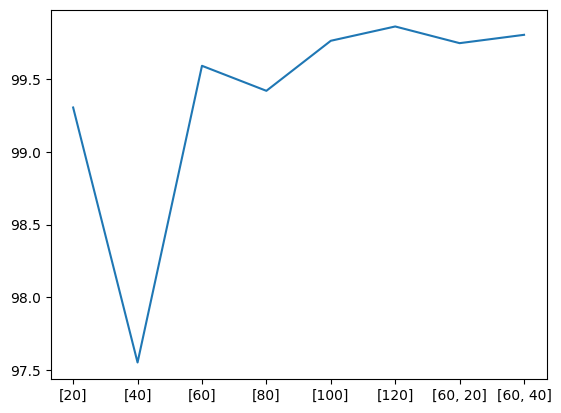
\includegraphics[width=0.6\textwidth]{Results/NeuronalNetwork/NN.png}
    \end{center}
 \end{figure}

\subsection{SVM}

Una Máquina de Vectores de Soporte (o SVM, por sus siglas en inglés), es un conjunto de algoritmos relacionados con problmas de clasificación y regresión. Una SVM intenta construir un hiperplano de un espacio N-dimensional que consiga clasificar los datos correctamente (donde N es el número de características que se proporcionan).

Entre las pruebas que realizamos, comparamos las que nos dieron los siguientes resultados:

{

\centering
\begin{tabular}{ |p{0.25cm}||p{0.75cm}|p{0.75cm}|p{3cm}|p{3cm}| p{3cm}|p{3cm}|  }
 \hline
 \multicolumn{7}{|c|}{Resultados obtenidos al aplicar SVM a nuestra base de datos.} \\
 \hline
    & C & Sigma & Porcentaje de datos usados (Training - Validation - Test) & Mejor probabilidad de acierto & Porcentaje de aciertos (\%) & Tiempo de análisis (s)\\
 \hline
 1 & 3.0 & 3.0 & 0.20 - 0.20 - 0.20 & 0.999 & 99.984 & 5572 \\
 2 & 3.0 & 3.0 & 0.20 - 0.20 - 0.20 & 0.999 & 99.984 & 3856 \\
 3 & 10.0 & 3.0 & 0.05 - 0.05 - 0.05 & 0.996 & 99.705 & 104 \\
 4 & 10.0 & 3.0 & 0.01 - 0.01 - 0.01 & 0.959 & 95.908 & 1.95 \\
 \hline
\end{tabular}
}

Entre las dos primeras pruebas que se muestran, es notable la diferencia de tiempos. Esto se debe a que, después de varias pruebas, decidimos utilizar hebras para agilizar este proceso. 

Entre los siguientes dos sets, el tiempo también se reduce dráticamente, pero por otro motivo: en estos casos, escogimos muestras más pequeñas para hacer las pruebas. Es interesante observar que, aunque el proceso es más rápido, el porcentaje de aciertos también decae.

Nuestro mejor resultado se corresponde, entonces, con la segunda entrada de la tabla: un 99.984\% de aciertos con un valor de C = 3.0 y un valor de sigma = 3.0, y reduciendo en casi 30 minutos el tiempo necesario para analizar los datos.

 \begin{figure}[H]
    \begin{center}
    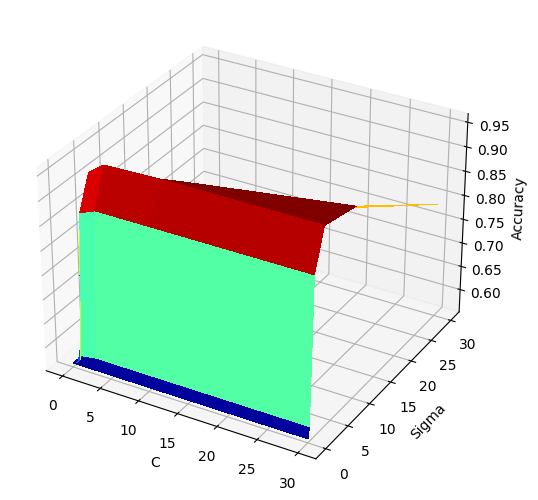
\includegraphics[width=0.75\textwidth]{Results/SVM/SVM_1.png}
    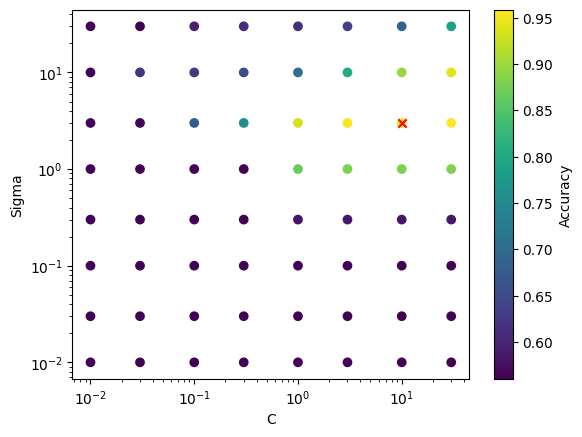
\includegraphics[width=0.75\textwidth]{Results/SVM/SVM_2.png}
    \end{center}
 \end{figure}

\newpage
\section{Conclusiones}

Para calcular los algoritmos, utilizamos en todos los casos unos datasets con las siguientes características:

\begin{itemize}
\item Tamaño de la muestra de entrenamiento: 12213 entradas
\item Tamaño de la muestra de validación: 12213 entradas
\item Tamaño de la muestra de testeo: 12213 entradas
\item En todos los casos, las muestras son diferentes entre sí. 
\end{itemize}

Tras realizar todas las pruebas, obtuvimos los siguientes resultados:

 \begin{figure}[H]
    \begin{center}
    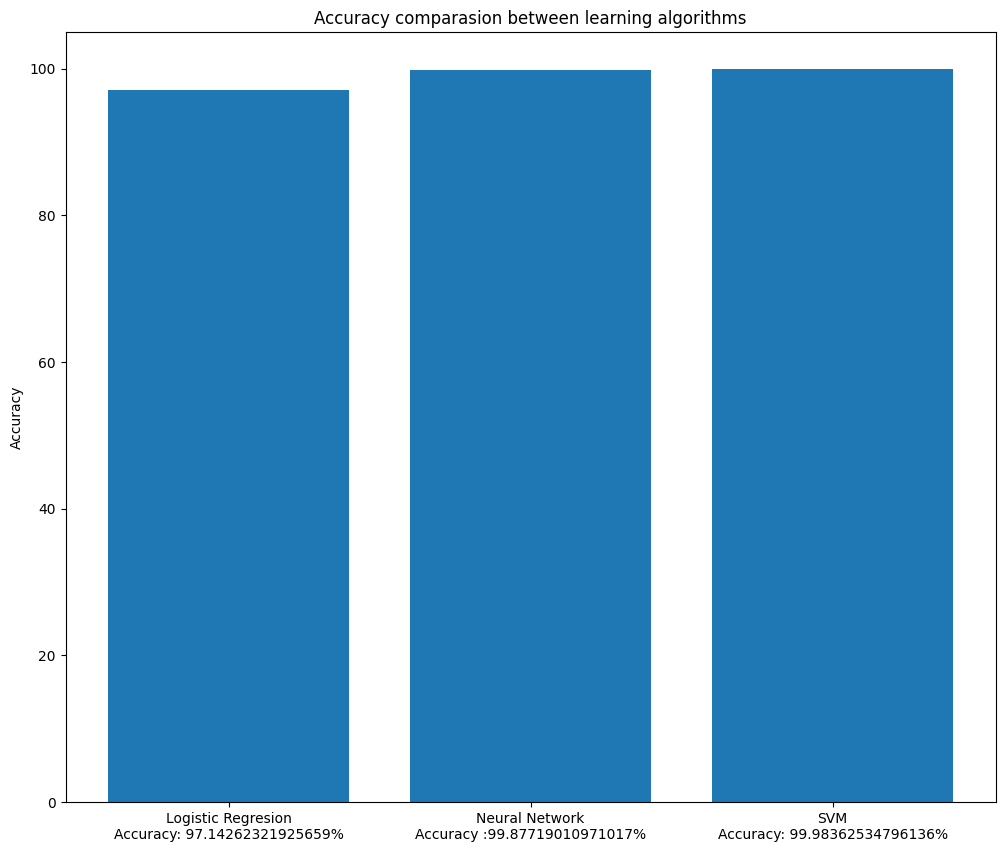
\includegraphics[width=\textwidth]{Results/FinalGraph.png}
    \end{center}
 \end{figure}
 
 \newpage
 \subsection{Implementación}
Para conseguir los resultados anteriores, implementamos las siguientes funciones, repartidas en varios archivos:


\lstinputlisting[language=Python]{src/evaluateLogistic.py}
\lstinputlisting[language=Python]{src/evaluateNeuronal.py}
\lstinputlisting[language=Python]{src/evaluateSVM.py}
\lstinputlisting[language=Python]{src/prepareData.py}
\lstinputlisting[language=Python]{src/threadRetVal.py}
\lstinputlisting[language=Python]{src/main.py}



\end{document}
